\documentclass[twoside]{book}

% Packages required by doxygen
\usepackage{fixltx2e}
\usepackage{calc}
\usepackage{doxygen}
\usepackage[export]{adjustbox} % also loads graphicx
\usepackage{graphicx}
\usepackage[utf8]{inputenc}
\usepackage{makeidx}
\usepackage{multicol}
\usepackage{multirow}
\PassOptionsToPackage{warn}{textcomp}
\usepackage{textcomp}
\usepackage[nointegrals]{wasysym}
\usepackage[table]{xcolor}

% Font selection
\usepackage[T1]{fontenc}
\usepackage[scaled=.90]{helvet}
\usepackage{courier}
\usepackage{amssymb}
\usepackage{sectsty}
\renewcommand{\familydefault}{\sfdefault}
\allsectionsfont{%
  \fontseries{bc}\selectfont%
  \color{darkgray}%
}
\renewcommand{\DoxyLabelFont}{%
  \fontseries{bc}\selectfont%
  \color{darkgray}%
}
\newcommand{\+}{\discretionary{\mbox{\scriptsize$\hookleftarrow$}}{}{}}

% Page & text layout
\usepackage{geometry}
\geometry{%
  a4paper,%
  top=2.5cm,%
  bottom=2.5cm,%
  left=2.5cm,%
  right=2.5cm%
}
\tolerance=750
\hfuzz=15pt
\hbadness=750
\setlength{\emergencystretch}{15pt}
\setlength{\parindent}{0cm}
\setlength{\parskip}{3ex plus 2ex minus 2ex}
\makeatletter
\renewcommand{\paragraph}{%
  \@startsection{paragraph}{4}{0ex}{-1.0ex}{1.0ex}{%
    \normalfont\normalsize\bfseries\SS@parafont%
  }%
}
\renewcommand{\subparagraph}{%
  \@startsection{subparagraph}{5}{0ex}{-1.0ex}{1.0ex}{%
    \normalfont\normalsize\bfseries\SS@subparafont%
  }%
}
\makeatother

% Headers & footers
\usepackage{fancyhdr}
\pagestyle{fancyplain}
\fancyhead[LE]{\fancyplain{}{\bfseries\thepage}}
\fancyhead[CE]{\fancyplain{}{}}
\fancyhead[RE]{\fancyplain{}{\bfseries\leftmark}}
\fancyhead[LO]{\fancyplain{}{\bfseries\rightmark}}
\fancyhead[CO]{\fancyplain{}{}}
\fancyhead[RO]{\fancyplain{}{\bfseries\thepage}}
\fancyfoot[LE]{\fancyplain{}{}}
\fancyfoot[CE]{\fancyplain{}{}}
\fancyfoot[RE]{\fancyplain{}{\bfseries\scriptsize Generated by Doxygen }}
\fancyfoot[LO]{\fancyplain{}{\bfseries\scriptsize Generated by Doxygen }}
\fancyfoot[CO]{\fancyplain{}{}}
\fancyfoot[RO]{\fancyplain{}{}}
\renewcommand{\footrulewidth}{0.4pt}
\renewcommand{\chaptermark}[1]{%
  \markboth{#1}{}%
}
\renewcommand{\sectionmark}[1]{%
  \markright{\thesection\ #1}%
}

% Indices & bibliography
\usepackage{natbib}
\usepackage[titles]{tocloft}
\setcounter{tocdepth}{3}
\setcounter{secnumdepth}{5}
\makeindex

% Hyperlinks (required, but should be loaded last)
\usepackage{ifpdf}
\ifpdf
  \usepackage[pdftex,pagebackref=true]{hyperref}
\else
  \usepackage[ps2pdf,pagebackref=true]{hyperref}
\fi
\hypersetup{%
  colorlinks=true,%
  linkcolor=blue,%
  citecolor=blue,%
  unicode%
}

% Custom commands
\newcommand{\clearemptydoublepage}{%
  \newpage{\pagestyle{empty}\cleardoublepage}%
}

\usepackage{caption}
\captionsetup{labelsep=space,justification=centering,font={bf},singlelinecheck=off,skip=4pt,position=top}

%===== C O N T E N T S =====

\begin{document}

% Titlepage & ToC
\hypersetup{pageanchor=false,
             bookmarksnumbered=true,
             pdfencoding=unicode
            }
\pagenumbering{alph}
\begin{titlepage}
\vspace*{7cm}
\begin{center}%
{\Large Drzewka }\\
\vspace*{1cm}
{\large Generated by Doxygen 1.8.13}\\
\end{center}
\end{titlepage}
\clearemptydoublepage
\pagenumbering{roman}
\tableofcontents
\clearemptydoublepage
\pagenumbering{arabic}
\hypersetup{pageanchor=true}

%--- Begin generated contents ---
\chapter{Hierarchical Index}
\section{Class Hierarchy}
This inheritance list is sorted roughly, but not completely, alphabetically\+:\begin{DoxyCompactList}
\item Action\+Listener\begin{DoxyCompactList}
\item \contentsline{section}{Window$<$ T extends Comparable$<$ T $>$}{\pageref{classWindow}}{}
\end{DoxyCompactList}
\item \contentsline{section}{Binary\+Tree$<$ T extends Comparable$<$ T $>$}{\pageref{classBinaryTree}}{}
\item \contentsline{section}{Binary\+Tree$<$ T $>$}{\pageref{classBinaryTree}}{}
\item J\+Frame\begin{DoxyCompactList}
\item \contentsline{section}{Window$<$ T extends Comparable$<$ T $>$}{\pageref{classWindow}}{}
\end{DoxyCompactList}
\item \contentsline{section}{Main}{\pageref{classMain}}{}
\item \contentsline{section}{Node$<$ T $>$}{\pageref{classNode}}{}
\item \contentsline{section}{Parser$<$ T $>$}{\pageref{classParser}}{}
\item \contentsline{section}{Parser\+Generic}{\pageref{interfaceParserGeneric}}{}
\begin{DoxyCompactList}
\item \contentsline{section}{Parser\+Double}{\pageref{classParserDouble}}{}
\item \contentsline{section}{Parser\+Integer}{\pageref{classParserInteger}}{}
\item \contentsline{section}{Parser\+String}{\pageref{classParserString}}{}
\end{DoxyCompactList}
\end{DoxyCompactList}

\chapter{Class Index}
\section{Class List}
Here are the classes, structs, unions and interfaces with brief descriptions\+:\begin{DoxyCompactList}
\item\contentsline{section}{\hyperlink{classBinaryTree}{Binary\+Tree$<$ T extends Comparable$<$ T $>$} }{\pageref{classBinaryTree}}{}
\item\contentsline{section}{\hyperlink{classMain}{Main} }{\pageref{classMain}}{}
\item\contentsline{section}{\hyperlink{classNode}{Node$<$ T $>$} }{\pageref{classNode}}{}
\item\contentsline{section}{\hyperlink{classParser}{Parser$<$ T $>$} }{\pageref{classParser}}{}
\item\contentsline{section}{\hyperlink{classParserDouble}{Parser\+Double} }{\pageref{classParserDouble}}{}
\item\contentsline{section}{\hyperlink{interfaceParserGeneric}{Parser\+Generic} }{\pageref{interfaceParserGeneric}}{}
\item\contentsline{section}{\hyperlink{classParserInteger}{Parser\+Integer} }{\pageref{classParserInteger}}{}
\item\contentsline{section}{\hyperlink{classParserString}{Parser\+String} }{\pageref{classParserString}}{}
\item\contentsline{section}{\hyperlink{classWindow}{Window$<$ T extends Comparable$<$ T $>$} }{\pageref{classWindow}}{}
\end{DoxyCompactList}

\chapter{File Index}
\section{File List}
Here is a list of all files with brief descriptions\+:\begin{DoxyCompactList}
\item\contentsline{section}{\hyperlink{BinaryTree_8java}{Binary\+Tree.\+java} }{\pageref{BinaryTree_8java}}{}
\item\contentsline{section}{\hyperlink{Main_8java}{Main.\+java} }{\pageref{Main_8java}}{}
\item\contentsline{section}{\hyperlink{Node_8java}{Node.\+java} }{\pageref{Node_8java}}{}
\item\contentsline{section}{\hyperlink{Parser_8java}{Parser.\+java} }{\pageref{Parser_8java}}{}
\item\contentsline{section}{\hyperlink{ParserDouble_8java}{Parser\+Double.\+java} }{\pageref{ParserDouble_8java}}{}
\item\contentsline{section}{\hyperlink{ParserGeneric_8java}{Parser\+Generic.\+java} }{\pageref{ParserGeneric_8java}}{}
\item\contentsline{section}{\hyperlink{ParserInteger_8java}{Parser\+Integer.\+java} }{\pageref{ParserInteger_8java}}{}
\item\contentsline{section}{\hyperlink{ParserString_8java}{Parser\+String.\+java} }{\pageref{ParserString_8java}}{}
\item\contentsline{section}{\hyperlink{Window_8java}{Window.\+java} }{\pageref{Window_8java}}{}
\end{DoxyCompactList}

\chapter{Class Documentation}
\hypertarget{classBinaryTree}{}\section{Binary\+Tree$<$ T $>$ Class Template Reference}
\label{classBinaryTree}\index{Binary\+Tree$<$ T $>$@{Binary\+Tree$<$ T $>$}}


{\ttfamily \#include $<$binary\+Tree.\+hpp$>$}

\subsection*{Public Member Functions}
\begin{DoxyCompactItemize}
\item 
\hyperlink{classBinaryTree_a9202cce23960faf8f647c6765decccd4}{Binary\+Tree} ()
\item 
void \hyperlink{classBinaryTree_ace861086e9b5510f32d04ad081500463}{add\+Node} (T key)
\item 
void \hyperlink{classBinaryTree_a547a4d22eb7a8f18ca09dd77402d88c6}{in\+Order} (\hyperlink{classNode}{Node}$<$ T $>$ $\ast$focus\+Node)
\item 
\hyperlink{classNode}{Node}$<$ T $>$ $\ast$ \hyperlink{classBinaryTree_a6110ff77e17b9f0db2170c8bead11210}{search} (T key)
\item 
void \hyperlink{classBinaryTree_a86fedb07a87af1b02e3408950c4f9663}{remove} (T key)
\item 
\hyperlink{classNode}{Node}$<$ T $>$ $\ast$ \hyperlink{classBinaryTree_a0055a6962c39301b5def80189be99601}{get\+Replacement\+Node} (\hyperlink{classNode}{Node}$<$ T $>$ $\ast$replaced\+Node)
\item 
\hyperlink{classNode}{Node}$<$ T $>$ $\ast$ \hyperlink{classBinaryTree_af525a78601eba600d880d1cd947a215a}{get\+Root} ()
\item 
void \hyperlink{classBinaryTree_a4653328dc7727b7c32285bb50a10f6c9}{delete\+Tree} (\hyperlink{classNode}{Node}$<$ T $>$ $\ast$node)
\item 
\hyperlink{classBinaryTree_a390c319c0b28b958463851119edb8af3}{$\sim$\+Binary\+Tree} ()
\end{DoxyCompactItemize}
\subsection*{Private Attributes}
\begin{DoxyCompactItemize}
\item 
\hyperlink{classNode}{Node}$<$ T $>$ $\ast$ \hyperlink{classBinaryTree_a2db40f59d96afceb1a005e6d9aef2374}{root}
\end{DoxyCompactItemize}


\subsection{Detailed Description}
\subsubsection*{template$<$typename T$>$\newline
class Binary\+Tree$<$ T $>$}

Klasa drzewa binarnego \begin{DoxySeeAlso}{See also}
Node$<$\+T$>$ 
\end{DoxySeeAlso}

\begin{DoxyTemplParams}{Template Parameters}
{\em Typ} & tworzonego drzewa \\
\hline
\end{DoxyTemplParams}


Definition at line 12 of file binary\+Tree.\+hpp.



\subsection{Constructor \& Destructor Documentation}
\mbox{\Hypertarget{classBinaryTree_a9202cce23960faf8f647c6765decccd4}\label{classBinaryTree_a9202cce23960faf8f647c6765decccd4}} 
\index{Binary\+Tree@{Binary\+Tree}!Binary\+Tree@{Binary\+Tree}}
\index{Binary\+Tree@{Binary\+Tree}!Binary\+Tree@{Binary\+Tree}}
\subsubsection{\texorpdfstring{Binary\+Tree()}{BinaryTree()}}
{\footnotesize\ttfamily template$<$typename T$>$ \\
\hyperlink{classBinaryTree}{Binary\+Tree}$<$ T $>$\+::\hyperlink{classBinaryTree}{Binary\+Tree} (\begin{DoxyParamCaption}{ }\end{DoxyParamCaption})\hspace{0.3cm}{\ttfamily [inline]}}

Konstruktor drzewa 

Definition at line 18 of file binary\+Tree.\+hpp.


\begin{DoxyCode}
18                      \{
19             \hyperlink{classBinaryTree_a2db40f59d96afceb1a005e6d9aef2374}{root} = NULL;
20         \}
\end{DoxyCode}
\mbox{\Hypertarget{classBinaryTree_a390c319c0b28b958463851119edb8af3}\label{classBinaryTree_a390c319c0b28b958463851119edb8af3}} 
\index{Binary\+Tree@{Binary\+Tree}!````~Binary\+Tree@{$\sim$\+Binary\+Tree}}
\index{````~Binary\+Tree@{$\sim$\+Binary\+Tree}!Binary\+Tree@{Binary\+Tree}}
\subsubsection{\texorpdfstring{$\sim$\+Binary\+Tree()}{~BinaryTree()}}
{\footnotesize\ttfamily template$<$typename T$>$ \\
\hyperlink{classBinaryTree}{Binary\+Tree}$<$ T $>$\+::$\sim$\hyperlink{classBinaryTree}{Binary\+Tree} (\begin{DoxyParamCaption}{ }\end{DoxyParamCaption})\hspace{0.3cm}{\ttfamily [inline]}}

Destruktor 

Definition at line 219 of file binary\+Tree.\+hpp.


\begin{DoxyCode}
219 \{\}
\end{DoxyCode}


\subsection{Member Function Documentation}
\mbox{\Hypertarget{classBinaryTree_ace861086e9b5510f32d04ad081500463}\label{classBinaryTree_ace861086e9b5510f32d04ad081500463}} 
\index{Binary\+Tree@{Binary\+Tree}!add\+Node@{add\+Node}}
\index{add\+Node@{add\+Node}!Binary\+Tree@{Binary\+Tree}}
\subsubsection{\texorpdfstring{add\+Node()}{addNode()}}
{\footnotesize\ttfamily template$<$typename T$>$ \\
void \hyperlink{classBinaryTree}{Binary\+Tree}$<$ T $>$\+::add\+Node (\begin{DoxyParamCaption}\item[{T}]{key }\end{DoxyParamCaption})\hspace{0.3cm}{\ttfamily [inline]}}

Metoda dodająca wierzchołek w drzewie 
\begin{DoxyParams}{Parameters}
{\em key} & Klucz który przypiszemy do nowego węzła \\
\hline
\end{DoxyParams}


Definition at line 25 of file binary\+Tree.\+hpp.


\begin{DoxyCode}
25                             \{
26             \hyperlink{classNode}{Node<T>} *node = \textcolor{keyword}{new} \hyperlink{classNode}{Node<T>}(key);
27 
28             \textcolor{keywordflow}{if}(\hyperlink{classBinaryTree_af525a78601eba600d880d1cd947a215a}{getRoot}() == NULL) \{
29                 \hyperlink{classBinaryTree_a2db40f59d96afceb1a005e6d9aef2374}{root} = node;
30                 \textcolor{keywordflow}{return};
31             \} \textcolor{keywordflow}{else} \{   
32 
33                 \hyperlink{classNode}{Node<T>} *focusNode = \hyperlink{classBinaryTree_a2db40f59d96afceb1a005e6d9aef2374}{root};
34                 \hyperlink{classNode}{Node<T>} *parent;
35 
36                 \textcolor{keywordflow}{while}(\textcolor{keyword}{true}) \{
37                     parent = focusNode;
38 
39                     \textcolor{keywordflow}{if} (key < focusNode->getKey()) \{
40                         focusNode = focusNode->\hyperlink{classNode_a1c884e62ef0a9b5dd4f35dbea09145f2}{getLeft}();
41                         \textcolor{keywordflow}{if} (focusNode == NULL) \{
42                             parent->\hyperlink{classNode_afc70e20117ea8083d11736f5ea8a9216}{setLeft}(node);
43                             \textcolor{keywordflow}{return};
44                         \}
45                     \}
46                     \textcolor{keywordflow}{else} \{
47                         focusNode = focusNode->\hyperlink{classNode_af9078f2651b16fc1a3502d7927761df1}{getRight}();
48                         \textcolor{keywordflow}{if} (focusNode == NULL) \{
49                             parent->\hyperlink{classNode_ad5c1f634547b3e2d03c3d55d355c0c17}{setRight}(node);
50                             \textcolor{keywordflow}{return};
51                         \}
52                     \}
53                 \}
54             \}
55         \}
\end{DoxyCode}
\mbox{\Hypertarget{classBinaryTree_a4653328dc7727b7c32285bb50a10f6c9}\label{classBinaryTree_a4653328dc7727b7c32285bb50a10f6c9}} 
\index{Binary\+Tree@{Binary\+Tree}!delete\+Tree@{delete\+Tree}}
\index{delete\+Tree@{delete\+Tree}!Binary\+Tree@{Binary\+Tree}}
\subsubsection{\texorpdfstring{delete\+Tree()}{deleteTree()}}
{\footnotesize\ttfamily template$<$typename T$>$ \\
void \hyperlink{classBinaryTree}{Binary\+Tree}$<$ T $>$\+::delete\+Tree (\begin{DoxyParamCaption}\item[{\hyperlink{classNode}{Node}$<$ T $>$ $\ast$}]{node }\end{DoxyParamCaption})\hspace{0.3cm}{\ttfamily [inline]}}

Metoda usuwa wszystkie wierzchołki drzewa 
\begin{DoxyParams}{Parameters}
{\em node} & Wierzchołek od którego zaczynamy usuwanie \\
\hline
\end{DoxyParams}


Definition at line 209 of file binary\+Tree.\+hpp.


\begin{DoxyCode}
209                                        \{  
210             \textcolor{keywordflow}{if} (node == NULL) \{ 
211                 \textcolor{keywordflow}{return};  
212             \}
213             \hyperlink{classBinaryTree_a4653328dc7727b7c32285bb50a10f6c9}{deleteTree}(node->\hyperlink{classNode_a2eaaeffaeef97da6291b788fa131c9ec}{leftChild});  
214             \hyperlink{classBinaryTree_a4653328dc7727b7c32285bb50a10f6c9}{deleteTree}(node->\hyperlink{classNode_a625cff56d169157a568afaedbb11576b}{rightChild});  
215             \textcolor{keyword}{delete} node; 
216         \} 
\end{DoxyCode}
\mbox{\Hypertarget{classBinaryTree_a0055a6962c39301b5def80189be99601}\label{classBinaryTree_a0055a6962c39301b5def80189be99601}} 
\index{Binary\+Tree@{Binary\+Tree}!get\+Replacement\+Node@{get\+Replacement\+Node}}
\index{get\+Replacement\+Node@{get\+Replacement\+Node}!Binary\+Tree@{Binary\+Tree}}
\subsubsection{\texorpdfstring{get\+Replacement\+Node()}{getReplacementNode()}}
{\footnotesize\ttfamily template$<$typename T$>$ \\
\hyperlink{classNode}{Node}$<$T$>$$\ast$ \hyperlink{classBinaryTree}{Binary\+Tree}$<$ T $>$\+::get\+Replacement\+Node (\begin{DoxyParamCaption}\item[{\hyperlink{classNode}{Node}$<$ T $>$ $\ast$}]{replaced\+Node }\end{DoxyParamCaption})\hspace{0.3cm}{\ttfamily [inline]}}

Metoda służąca do zastępowania usuwanego wierzchołka 
\begin{DoxyParams}{Parameters}
{\em replaced\+Node} & Usuwany wierzchołek \\
\hline
\end{DoxyParams}
\begin{DoxyReturn}{Returns}
Wierzchołek którym zastąpimy usuwany wierzchołek 
\end{DoxyReturn}


Definition at line 180 of file binary\+Tree.\+hpp.


\begin{DoxyCode}
180                                                            \{
181             \hyperlink{classNode}{Node<T>} *replacementParent = replacedNode;
182             \hyperlink{classNode}{Node<T>} *replacement = replacedNode;
183             \hyperlink{classNode}{Node<T>} *focusNode = replacedNode->\hyperlink{classNode_af9078f2651b16fc1a3502d7927761df1}{getRight}();
184 
185             \textcolor{keywordflow}{while} (focusNode != NULL) \{
186                 replacementParent = replacement;
187                 replacement = focusNode;
188                 focusNode = focusNode->\hyperlink{classNode_a1c884e62ef0a9b5dd4f35dbea09145f2}{getLeft}();
189             \}
190 
191             \textcolor{keywordflow}{if} (replacement != replacedNode->\hyperlink{classNode_af9078f2651b16fc1a3502d7927761df1}{getRight}()) \{
192                 replacementParent->\hyperlink{classNode_afc70e20117ea8083d11736f5ea8a9216}{setLeft}(replacement->\hyperlink{classNode_af9078f2651b16fc1a3502d7927761df1}{getRight}());
193                 replacement->\hyperlink{classNode_ad5c1f634547b3e2d03c3d55d355c0c17}{setRight}(replacedNode->\hyperlink{classNode_af9078f2651b16fc1a3502d7927761df1}{getRight}());
194             \}
195 
196             \textcolor{keyword}{delete} replacementParent;
197             \textcolor{keyword}{delete} focusNode;
198             \textcolor{keywordflow}{return} replacement;
199         \}
\end{DoxyCode}
\mbox{\Hypertarget{classBinaryTree_af525a78601eba600d880d1cd947a215a}\label{classBinaryTree_af525a78601eba600d880d1cd947a215a}} 
\index{Binary\+Tree@{Binary\+Tree}!get\+Root@{get\+Root}}
\index{get\+Root@{get\+Root}!Binary\+Tree@{Binary\+Tree}}
\subsubsection{\texorpdfstring{get\+Root()}{getRoot()}}
{\footnotesize\ttfamily template$<$typename T$>$ \\
\hyperlink{classNode}{Node}$<$T$>$$\ast$ \hyperlink{classBinaryTree}{Binary\+Tree}$<$ T $>$\+::get\+Root (\begin{DoxyParamCaption}{ }\end{DoxyParamCaption})\hspace{0.3cm}{\ttfamily [inline]}}

Metoda zwraca korzeń drzewa \begin{DoxyReturn}{Returns}
Korzeń drzewa 
\end{DoxyReturn}


Definition at line 203 of file binary\+Tree.\+hpp.


\begin{DoxyCode}
203                            \{
204             \textcolor{keywordflow}{return} \hyperlink{classBinaryTree_a2db40f59d96afceb1a005e6d9aef2374}{root};
205         \}
\end{DoxyCode}
\mbox{\Hypertarget{classBinaryTree_a547a4d22eb7a8f18ca09dd77402d88c6}\label{classBinaryTree_a547a4d22eb7a8f18ca09dd77402d88c6}} 
\index{Binary\+Tree@{Binary\+Tree}!in\+Order@{in\+Order}}
\index{in\+Order@{in\+Order}!Binary\+Tree@{Binary\+Tree}}
\subsubsection{\texorpdfstring{in\+Order()}{inOrder()}}
{\footnotesize\ttfamily template$<$typename T$>$ \\
void \hyperlink{classBinaryTree}{Binary\+Tree}$<$ T $>$\+::in\+Order (\begin{DoxyParamCaption}\item[{\hyperlink{classNode}{Node}$<$ T $>$ $\ast$}]{focus\+Node }\end{DoxyParamCaption})\hspace{0.3cm}{\ttfamily [inline]}}

Metoda drukująca drzewo metodą inorder 
\begin{DoxyParams}{Parameters}
{\em focus\+Node} & Wierzchołek od którego zaczynamy wypisywanie \\
\hline
\end{DoxyParams}
rekurencyjnie uruchamiamy metodę dla lewego poddrzewa

Następnie wywołujemy metodę dla prawego poddrzewa 

Definition at line 59 of file binary\+Tree.\+hpp.


\begin{DoxyCode}
59                                          \{
60            \textcolor{keywordflow}{if} (focusNode->\hyperlink{classNode_a906ae0e0b015275eacf168ef55017f7f}{isLeft}()) \{
61                std::cout << \textcolor{stringliteral}{"("};
63                \hyperlink{classBinaryTree_a547a4d22eb7a8f18ca09dd77402d88c6}{inOrder}(focusNode->\hyperlink{classNode_a1c884e62ef0a9b5dd4f35dbea09145f2}{getLeft}());
64                std::cout << \textcolor{stringliteral}{")"};
65            \}
66            std::cout << focusNode->\hyperlink{classNode_a3c04afa4e4c8e555cc87a22757ab5f6a}{getKey}();
67            \textcolor{keywordflow}{if} (focusNode->\hyperlink{classNode_a983178a46cc464ca0738ee8c7d8b2cc4}{isRight}()) \{
68                std::cout << \textcolor{stringliteral}{"("};
70                \hyperlink{classBinaryTree_a547a4d22eb7a8f18ca09dd77402d88c6}{inOrder}(focusNode->\hyperlink{classNode_af9078f2651b16fc1a3502d7927761df1}{getRight}());
71                std::cout << \textcolor{stringliteral}{")"};
72            \}
73         \}
\end{DoxyCode}
\mbox{\Hypertarget{classBinaryTree_a86fedb07a87af1b02e3408950c4f9663}\label{classBinaryTree_a86fedb07a87af1b02e3408950c4f9663}} 
\index{Binary\+Tree@{Binary\+Tree}!remove@{remove}}
\index{remove@{remove}!Binary\+Tree@{Binary\+Tree}}
\subsubsection{\texorpdfstring{remove()}{remove()}}
{\footnotesize\ttfamily template$<$typename T$>$ \\
void \hyperlink{classBinaryTree}{Binary\+Tree}$<$ T $>$\+::remove (\begin{DoxyParamCaption}\item[{T}]{key }\end{DoxyParamCaption})\hspace{0.3cm}{\ttfamily [inline]}}

Metoda usuwająca wierzchołek z drzewa 
\begin{DoxyParams}{Parameters}
{\em key} & Klucz który chcemy w drzewa usunąć \\
\hline
\end{DoxyParams}
Szukamy wierzchołka o podanym kluczu

Sprawdzamy, czy dany wierzchołek ma potomków aby złożyć drzewo w całość

W przypadku, gdy drzewo ma oboje potomków wywołujemy metodę get\+Replacement\+Node 

Definition at line 102 of file binary\+Tree.\+hpp.


\begin{DoxyCode}
102                            \{
103             \textcolor{keywordflow}{if} (\hyperlink{classBinaryTree_a2db40f59d96afceb1a005e6d9aef2374}{root} == NULL) \{
104                 \textcolor{keywordflow}{return};
105             \}
106 
107             \hyperlink{classNode}{Node<T>} *ptr = \hyperlink{classBinaryTree_a2db40f59d96afceb1a005e6d9aef2374}{root};
108             \hyperlink{classNode}{Node<T>} *parent = \hyperlink{classBinaryTree_a2db40f59d96afceb1a005e6d9aef2374}{root};
109             \textcolor{keywordtype}{bool} isItALeftChild = \textcolor{keyword}{true};
110 
112             \textcolor{keywordflow}{while} (ptr->\hyperlink{classNode_a3c04afa4e4c8e555cc87a22757ab5f6a}{getKey}() != key) \{
113                 parent = ptr;
114 
115                 \textcolor{keywordflow}{if} (key < ptr->getKey()) \{
116                     isItALeftChild = \textcolor{keyword}{true};
117                     ptr = ptr->\hyperlink{classNode_a1c884e62ef0a9b5dd4f35dbea09145f2}{getLeft}();
118                 \}
119                 \textcolor{keywordflow}{else} \{
120                     isItALeftChild = \textcolor{keyword}{false};
121                     ptr = ptr->\hyperlink{classNode_af9078f2651b16fc1a3502d7927761df1}{getRight}();
122                 \}
123 
124                 \textcolor{keywordflow}{if} (ptr == NULL) \{
125                     \textcolor{keywordflow}{return};
126                 \}
127             \}
128 
130             \textcolor{keywordflow}{if} (!ptr->\hyperlink{classNode_a906ae0e0b015275eacf168ef55017f7f}{isLeft}() && !ptr->\hyperlink{classNode_a983178a46cc464ca0738ee8c7d8b2cc4}{isRight}()) \{
131                 \textcolor{keywordflow}{if} (ptr == \hyperlink{classBinaryTree_a2db40f59d96afceb1a005e6d9aef2374}{root}) \{
132                     \hyperlink{classBinaryTree_a2db40f59d96afceb1a005e6d9aef2374}{root} = NULL;    
133                 \} \textcolor{keywordflow}{else} \textcolor{keywordflow}{if} (isItALeftChild) \{
134                     parent->\hyperlink{classNode_afc70e20117ea8083d11736f5ea8a9216}{setLeft}(NULL);
135                 \} \textcolor{keywordflow}{else} \{
136                     parent->\hyperlink{classNode_ad5c1f634547b3e2d03c3d55d355c0c17}{setRight}(NULL);
137                 \}
138             \}
139                     
140             \textcolor{keywordflow}{else} \textcolor{keywordflow}{if} (!ptr->\hyperlink{classNode_a983178a46cc464ca0738ee8c7d8b2cc4}{isRight}()) \{
141                 \textcolor{keywordflow}{if} (ptr == \hyperlink{classBinaryTree_a2db40f59d96afceb1a005e6d9aef2374}{root}) \{
142                     \hyperlink{classBinaryTree_a2db40f59d96afceb1a005e6d9aef2374}{root} = ptr->\hyperlink{classNode_a1c884e62ef0a9b5dd4f35dbea09145f2}{getLeft}();
143                 \} \textcolor{keywordflow}{else} \textcolor{keywordflow}{if} (isItALeftChild) \{
144                         parent->\hyperlink{classNode_afc70e20117ea8083d11736f5ea8a9216}{setLeft}(ptr->\hyperlink{classNode_a1c884e62ef0a9b5dd4f35dbea09145f2}{getLeft}());
145                 \} \textcolor{keywordflow}{else} \{
146                     parent->\hyperlink{classNode_ad5c1f634547b3e2d03c3d55d355c0c17}{setRight}(ptr->\hyperlink{classNode_a1c884e62ef0a9b5dd4f35dbea09145f2}{getLeft}());
147                 \}
148             \}
149 
150             \textcolor{keywordflow}{else} \textcolor{keywordflow}{if} (!ptr->\hyperlink{classNode_a906ae0e0b015275eacf168ef55017f7f}{isLeft}()) \{
151                 \textcolor{keywordflow}{if} (ptr == \hyperlink{classBinaryTree_a2db40f59d96afceb1a005e6d9aef2374}{root}) \{
152                     \hyperlink{classBinaryTree_a2db40f59d96afceb1a005e6d9aef2374}{root} = ptr->\hyperlink{classNode_af9078f2651b16fc1a3502d7927761df1}{getRight}();
153                 \} \textcolor{keywordflow}{else} \textcolor{keywordflow}{if} (isItALeftChild) \{
154                     parent->\hyperlink{classNode_afc70e20117ea8083d11736f5ea8a9216}{setLeft}(ptr->\hyperlink{classNode_af9078f2651b16fc1a3502d7927761df1}{getRight}());
155                 \} \textcolor{keywordflow}{else} \{
156                     parent->\hyperlink{classNode_afc70e20117ea8083d11736f5ea8a9216}{setLeft}(ptr->\hyperlink{classNode_af9078f2651b16fc1a3502d7927761df1}{getRight}());
157                 \}
158             \}
159 
161             \textcolor{keywordflow}{else} \{
162                 \hyperlink{classNode}{Node<T>} *replacement = \hyperlink{classBinaryTree_a0055a6962c39301b5def80189be99601}{getReplacementNode}(ptr);
163 
164                 \textcolor{keywordflow}{if} (ptr == \hyperlink{classBinaryTree_a2db40f59d96afceb1a005e6d9aef2374}{root}) \{
165                     \hyperlink{classBinaryTree_a2db40f59d96afceb1a005e6d9aef2374}{root} = replacement;
166                 \} \textcolor{keywordflow}{else} \textcolor{keywordflow}{if} (isItALeftChild) \{
167                     parent->\hyperlink{classNode_afc70e20117ea8083d11736f5ea8a9216}{setLeft}(replacement);
168                 \} \textcolor{keywordflow}{else} \{
169                     parent->\hyperlink{classNode_ad5c1f634547b3e2d03c3d55d355c0c17}{setRight}(replacement);
170                 \}
171 
172                 replacement->\hyperlink{classNode_afc70e20117ea8083d11736f5ea8a9216}{setLeft}(ptr->\hyperlink{classNode_a1c884e62ef0a9b5dd4f35dbea09145f2}{getLeft}());
173             \}
174 
175         \}
\end{DoxyCode}
\mbox{\Hypertarget{classBinaryTree_a6110ff77e17b9f0db2170c8bead11210}\label{classBinaryTree_a6110ff77e17b9f0db2170c8bead11210}} 
\index{Binary\+Tree@{Binary\+Tree}!search@{search}}
\index{search@{search}!Binary\+Tree@{Binary\+Tree}}
\subsubsection{\texorpdfstring{search()}{search()}}
{\footnotesize\ttfamily template$<$typename T$>$ \\
\hyperlink{classNode}{Node}$<$T$>$$\ast$ \hyperlink{classBinaryTree}{Binary\+Tree}$<$ T $>$\+::search (\begin{DoxyParamCaption}\item[{T}]{key }\end{DoxyParamCaption})\hspace{0.3cm}{\ttfamily [inline]}}

Metoda szukająca wierzchołka o danym kluczu 
\begin{DoxyParams}{Parameters}
{\em key} & Klucz, dla którego szukamy wierzchołek \\
\hline
\end{DoxyParams}
\begin{DoxyReturn}{Returns}
Wierzchołęk o podanym kluczu lub N\+U\+LL 
\end{DoxyReturn}


Definition at line 78 of file binary\+Tree.\+hpp.


\begin{DoxyCode}
78                                \{
79             \textcolor{keywordflow}{if} (\hyperlink{classBinaryTree_a2db40f59d96afceb1a005e6d9aef2374}{root} == NULL) \{
80                 \textcolor{keywordflow}{return} NULL;
81             \}
82 
83             \hyperlink{classNode}{Node<T>}* focusNode = \hyperlink{classBinaryTree_a2db40f59d96afceb1a005e6d9aef2374}{root};
84 
85             \textcolor{keywordflow}{while} (focusNode->\hyperlink{classNode_a3c04afa4e4c8e555cc87a22757ab5f6a}{getKey}() != key) \{
86                 \textcolor{keywordflow}{if} (key < focusNode->getKey()) \{
87                     focusNode = focusNode->\hyperlink{classNode_a2eaaeffaeef97da6291b788fa131c9ec}{leftChild};
88                 \} \textcolor{keywordflow}{else} \{
89                     focusNode = focusNode->\hyperlink{classNode_a625cff56d169157a568afaedbb11576b}{rightChild};
90                 \}
91 
92                 \textcolor{keywordflow}{if} (focusNode == NULL) \{
93                     \textcolor{keywordflow}{return} NULL;
94                 \}
95             \}
96 
97             \textcolor{keywordflow}{return} focusNode;
98         \}
\end{DoxyCode}


\subsection{Member Data Documentation}
\mbox{\Hypertarget{classBinaryTree_a2db40f59d96afceb1a005e6d9aef2374}\label{classBinaryTree_a2db40f59d96afceb1a005e6d9aef2374}} 
\index{Binary\+Tree@{Binary\+Tree}!root@{root}}
\index{root@{root}!Binary\+Tree@{Binary\+Tree}}
\subsubsection{\texorpdfstring{root}{root}}
{\footnotesize\ttfamily template$<$typename T$>$ \\
\hyperlink{classNode}{Node}$<$T$>$$\ast$ \hyperlink{classBinaryTree}{Binary\+Tree}$<$ T $>$\+::root\hspace{0.3cm}{\ttfamily [private]}}

Wierzchołek drzewa 

Definition at line 15 of file binary\+Tree.\+hpp.



The documentation for this class was generated from the following file\+:\begin{DoxyCompactItemize}
\item 
binary\+Tree.\+hpp\end{DoxyCompactItemize}

\hypertarget{classMain}{}\section{Main Class Reference}
\label{classMain}\index{Main@{Main}}
\subsection*{Static Public Member Functions}
\begin{DoxyCompactItemize}
\item 
static void \hyperlink{classMain_a8a5d0f827edddff706cc0e6740d0579a}{main} (String\mbox{[}$\,$\mbox{]} args)
\end{DoxyCompactItemize}


\subsection{Detailed Description}
Klasa uruchamiająca program \char`\"{}\+Drzewka\char`\"{} \begin{DoxyAuthor}{Author}
Wojciech Strzelecki 
\end{DoxyAuthor}
\begin{DoxyVersion}{Version}
1.\+0 
\end{DoxyVersion}
\begin{DoxySince}{Since}
13.\+06.\+2020 
\end{DoxySince}
\begin{DoxySeeAlso}{See also}
\hyperlink{classWindow}{Window} 
\end{DoxySeeAlso}


\subsection{Member Function Documentation}
\mbox{\Hypertarget{classMain_a8a5d0f827edddff706cc0e6740d0579a}\label{classMain_a8a5d0f827edddff706cc0e6740d0579a}} 
\index{Main@{Main}!main@{main}}
\index{main@{main}!Main@{Main}}
\subsubsection{\texorpdfstring{main()}{main()}}
{\footnotesize\ttfamily static void Main.\+main (\begin{DoxyParamCaption}\item[{String \mbox{[}$\,$\mbox{]}}]{args }\end{DoxyParamCaption})\hspace{0.3cm}{\ttfamily [inline]}, {\ttfamily [static]}}

Tworzymy wskaźnik na drzewo danego typu

W zależności od wybranego typu tworzymy drzewo tego typu 

The documentation for this class was generated from the following file\+:\begin{DoxyCompactItemize}
\item 
\hyperlink{Main_8java}{Main.\+java}\end{DoxyCompactItemize}

\hypertarget{classNode}{}\section{Node$<$ T $>$ Class Template Reference}
\label{classNode}\index{Node$<$ T $>$@{Node$<$ T $>$}}


{\ttfamily \#include $<$node.\+hpp$>$}

\subsection*{Public Member Functions}
\begin{DoxyCompactItemize}
\item 
\hyperlink{classNode_a46dceddf91d9d3c68f941333ae1a7dc1}{Node} (T \hyperlink{classNode_a9d5e5c1914f5ed67389740354a607527}{key})
\item 
T \hyperlink{classNode_a3c04afa4e4c8e555cc87a22757ab5f6a}{get\+Key} ()
\item 
void \hyperlink{classNode_afc70e20117ea8083d11736f5ea8a9216}{set\+Left} (\hyperlink{classNode}{Node}$<$ T $>$ $\ast$l)
\item 
void \hyperlink{classNode_ad5c1f634547b3e2d03c3d55d355c0c17}{set\+Right} (\hyperlink{classNode}{Node}$<$ T $>$ $\ast$r)
\item 
void \hyperlink{classNode_a3162a541ae436cd98d61750f07f274b2}{set\+Key} (T d)
\item 
bool \hyperlink{classNode_a906ae0e0b015275eacf168ef55017f7f}{is\+Left} ()
\item 
bool \hyperlink{classNode_a983178a46cc464ca0738ee8c7d8b2cc4}{is\+Right} ()
\item 
\hyperlink{classNode}{Node}$<$ T $>$ $\ast$ \hyperlink{classNode_a1c884e62ef0a9b5dd4f35dbea09145f2}{get\+Left} ()
\item 
\hyperlink{classNode}{Node}$<$ T $>$ $\ast$ \hyperlink{classNode_af9078f2651b16fc1a3502d7927761df1}{get\+Right} ()
\item 
\hyperlink{classNode_ae923d0417581dd19784d55b901f0f7f0}{$\sim$\+Node} ()
\end{DoxyCompactItemize}
\subsection*{Public Attributes}
\begin{DoxyCompactItemize}
\item 
\hyperlink{classNode}{Node}$<$ T $>$ $\ast$ \hyperlink{classNode_a2eaaeffaeef97da6291b788fa131c9ec}{left\+Child}
\item 
\hyperlink{classNode}{Node}$<$ T $>$ $\ast$ \hyperlink{classNode_a625cff56d169157a568afaedbb11576b}{right\+Child}
\end{DoxyCompactItemize}
\subsection*{Private Attributes}
\begin{DoxyCompactItemize}
\item 
T \hyperlink{classNode_a9d5e5c1914f5ed67389740354a607527}{key}
\end{DoxyCompactItemize}


\subsection{Detailed Description}
\subsubsection*{template$<$typename T$>$\newline
class Node$<$ T $>$}

Klasa wierzchołka w drzewie 
\begin{DoxyTemplParams}{Template Parameters}
{\em Typ} & klucza wierzchołka \\
\hline
\end{DoxyTemplParams}


Definition at line 9 of file node.\+hpp.



\subsection{Constructor \& Destructor Documentation}
\mbox{\Hypertarget{classNode_a46dceddf91d9d3c68f941333ae1a7dc1}\label{classNode_a46dceddf91d9d3c68f941333ae1a7dc1}} 
\index{Node@{Node}!Node@{Node}}
\index{Node@{Node}!Node@{Node}}
\subsubsection{\texorpdfstring{Node()}{Node()}}
{\footnotesize\ttfamily template$<$typename T$>$ \\
\hyperlink{classNode}{Node}$<$ T $>$\+::\hyperlink{classNode}{Node} (\begin{DoxyParamCaption}\item[{T}]{key }\end{DoxyParamCaption})\hspace{0.3cm}{\ttfamily [inline]}}

Konstruktor 
\begin{DoxyParams}{Parameters}
{\em key} & Klucz \\
\hline
\end{DoxyParams}


Definition at line 21 of file node.\+hpp.


\begin{DoxyCode}
21                     \{
22             this->\hyperlink{classNode_a9d5e5c1914f5ed67389740354a607527}{key} = \hyperlink{classNode_a9d5e5c1914f5ed67389740354a607527}{key};
23         \}
\end{DoxyCode}
\mbox{\Hypertarget{classNode_ae923d0417581dd19784d55b901f0f7f0}\label{classNode_ae923d0417581dd19784d55b901f0f7f0}} 
\index{Node@{Node}!````~Node@{$\sim$\+Node}}
\index{````~Node@{$\sim$\+Node}!Node@{Node}}
\subsubsection{\texorpdfstring{$\sim$\+Node()}{~Node()}}
{\footnotesize\ttfamily template$<$typename T$>$ \\
\hyperlink{classNode}{Node}$<$ T $>$\+::$\sim$\hyperlink{classNode}{Node} (\begin{DoxyParamCaption}{ }\end{DoxyParamCaption})\hspace{0.3cm}{\ttfamily [inline]}}

Destruktor 

Definition at line 80 of file node.\+hpp.


\begin{DoxyCode}
80 \{\}
\end{DoxyCode}


\subsection{Member Function Documentation}
\mbox{\Hypertarget{classNode_a3c04afa4e4c8e555cc87a22757ab5f6a}\label{classNode_a3c04afa4e4c8e555cc87a22757ab5f6a}} 
\index{Node@{Node}!get\+Key@{get\+Key}}
\index{get\+Key@{get\+Key}!Node@{Node}}
\subsubsection{\texorpdfstring{get\+Key()}{getKey()}}
{\footnotesize\ttfamily template$<$typename T$>$ \\
T \hyperlink{classNode}{Node}$<$ T $>$\+::get\+Key (\begin{DoxyParamCaption}{ }\end{DoxyParamCaption})\hspace{0.3cm}{\ttfamily [inline]}}

Metoda zwracjąca klucz \begin{DoxyReturn}{Returns}
Klucz wierzchołka 
\end{DoxyReturn}


Definition at line 27 of file node.\+hpp.


\begin{DoxyCode}
27                    \{
28             \textcolor{keywordflow}{return} \hyperlink{classNode_a9d5e5c1914f5ed67389740354a607527}{key};
29         \}
\end{DoxyCode}
\mbox{\Hypertarget{classNode_a1c884e62ef0a9b5dd4f35dbea09145f2}\label{classNode_a1c884e62ef0a9b5dd4f35dbea09145f2}} 
\index{Node@{Node}!get\+Left@{get\+Left}}
\index{get\+Left@{get\+Left}!Node@{Node}}
\subsubsection{\texorpdfstring{get\+Left()}{getLeft()}}
{\footnotesize\ttfamily template$<$typename T$>$ \\
\hyperlink{classNode}{Node}$<$T$>$$\ast$ \hyperlink{classNode}{Node}$<$ T $>$\+::get\+Left (\begin{DoxyParamCaption}{ }\end{DoxyParamCaption})\hspace{0.3cm}{\ttfamily [inline]}}

Metoda zwracająca wskaźnik na lewego syna \begin{DoxyReturn}{Returns}
Wskaźnik na lewego syna 
\end{DoxyReturn}


Definition at line 69 of file node.\+hpp.


\begin{DoxyCode}
69                            \{
70              \textcolor{keywordflow}{return} \hyperlink{classNode_a2eaaeffaeef97da6291b788fa131c9ec}{leftChild};
71         \}
\end{DoxyCode}
\mbox{\Hypertarget{classNode_af9078f2651b16fc1a3502d7927761df1}\label{classNode_af9078f2651b16fc1a3502d7927761df1}} 
\index{Node@{Node}!get\+Right@{get\+Right}}
\index{get\+Right@{get\+Right}!Node@{Node}}
\subsubsection{\texorpdfstring{get\+Right()}{getRight()}}
{\footnotesize\ttfamily template$<$typename T$>$ \\
\hyperlink{classNode}{Node}$<$T$>$$\ast$ \hyperlink{classNode}{Node}$<$ T $>$\+::get\+Right (\begin{DoxyParamCaption}{ }\end{DoxyParamCaption})\hspace{0.3cm}{\ttfamily [inline]}}

Metoda zwracająca wskaźnik na prawego syna \begin{DoxyReturn}{Returns}
Wskaźnik na prawego syna 
\end{DoxyReturn}


Definition at line 75 of file node.\+hpp.


\begin{DoxyCode}
75                             \{
76              \textcolor{keywordflow}{return} \hyperlink{classNode_a625cff56d169157a568afaedbb11576b}{rightChild};
77         \}
\end{DoxyCode}
\mbox{\Hypertarget{classNode_a906ae0e0b015275eacf168ef55017f7f}\label{classNode_a906ae0e0b015275eacf168ef55017f7f}} 
\index{Node@{Node}!is\+Left@{is\+Left}}
\index{is\+Left@{is\+Left}!Node@{Node}}
\subsubsection{\texorpdfstring{is\+Left()}{isLeft()}}
{\footnotesize\ttfamily template$<$typename T$>$ \\
bool \hyperlink{classNode}{Node}$<$ T $>$\+::is\+Left (\begin{DoxyParamCaption}{ }\end{DoxyParamCaption})\hspace{0.3cm}{\ttfamily [inline]}}

Metoda sprawdzająca czy wierzchołek ma lewego syna \begin{DoxyReturn}{Returns}
Prawdę, jeśli lewy syn istnieje. W przeciwnym wypadku fałsz 
\end{DoxyReturn}


Definition at line 51 of file node.\+hpp.


\begin{DoxyCode}
51                       \{
52             \textcolor{keywordflow}{if}(\hyperlink{classNode_a2eaaeffaeef97da6291b788fa131c9ec}{leftChild} == NULL) \{
53                 \textcolor{keywordflow}{return} \textcolor{keyword}{false};
54             \}
55             \textcolor{keywordflow}{return} \textcolor{keyword}{true};
56         \}
\end{DoxyCode}
\mbox{\Hypertarget{classNode_a983178a46cc464ca0738ee8c7d8b2cc4}\label{classNode_a983178a46cc464ca0738ee8c7d8b2cc4}} 
\index{Node@{Node}!is\+Right@{is\+Right}}
\index{is\+Right@{is\+Right}!Node@{Node}}
\subsubsection{\texorpdfstring{is\+Right()}{isRight()}}
{\footnotesize\ttfamily template$<$typename T$>$ \\
bool \hyperlink{classNode}{Node}$<$ T $>$\+::is\+Right (\begin{DoxyParamCaption}{ }\end{DoxyParamCaption})\hspace{0.3cm}{\ttfamily [inline]}}

Metoda sprawdzająca czy wierzchołek ma prawego syna \begin{DoxyReturn}{Returns}
Prawdę, jeśli prawy syn istnieje. W przeciwnym wypadku fałsz 
\end{DoxyReturn}


Definition at line 60 of file node.\+hpp.


\begin{DoxyCode}
60                        \{
61             \textcolor{keywordflow}{if}(\hyperlink{classNode_a625cff56d169157a568afaedbb11576b}{rightChild} == NULL) \{
62                 \textcolor{keywordflow}{return} \textcolor{keyword}{false};
63             \}
64             \textcolor{keywordflow}{return} \textcolor{keyword}{true};
65         \}
\end{DoxyCode}
\mbox{\Hypertarget{classNode_a3162a541ae436cd98d61750f07f274b2}\label{classNode_a3162a541ae436cd98d61750f07f274b2}} 
\index{Node@{Node}!set\+Key@{set\+Key}}
\index{set\+Key@{set\+Key}!Node@{Node}}
\subsubsection{\texorpdfstring{set\+Key()}{setKey()}}
{\footnotesize\ttfamily template$<$typename T$>$ \\
void \hyperlink{classNode}{Node}$<$ T $>$\+::set\+Key (\begin{DoxyParamCaption}\item[{T}]{d }\end{DoxyParamCaption})\hspace{0.3cm}{\ttfamily [inline]}}

Metoda ustawiająca nową wartość klucza 
\begin{DoxyParams}{Parameters}
{\em d} & Nowy klucz \\
\hline
\end{DoxyParams}


Definition at line 45 of file node.\+hpp.


\begin{DoxyCode}
45                          \{
46             \hyperlink{classNode_a9d5e5c1914f5ed67389740354a607527}{key} = d;
47         \}
\end{DoxyCode}
\mbox{\Hypertarget{classNode_afc70e20117ea8083d11736f5ea8a9216}\label{classNode_afc70e20117ea8083d11736f5ea8a9216}} 
\index{Node@{Node}!set\+Left@{set\+Left}}
\index{set\+Left@{set\+Left}!Node@{Node}}
\subsubsection{\texorpdfstring{set\+Left()}{setLeft()}}
{\footnotesize\ttfamily template$<$typename T$>$ \\
void \hyperlink{classNode}{Node}$<$ T $>$\+::set\+Left (\begin{DoxyParamCaption}\item[{\hyperlink{classNode}{Node}$<$ T $>$ $\ast$}]{l }\end{DoxyParamCaption})\hspace{0.3cm}{\ttfamily [inline]}}

Metoda ustawiająca nowego lewego potomka 
\begin{DoxyParams}{Parameters}
{\em l} & Wskaźnik na nowego potomka \\
\hline
\end{DoxyParams}


Definition at line 33 of file node.\+hpp.


\begin{DoxyCode}
33                                  \{
34             \hyperlink{classNode_a2eaaeffaeef97da6291b788fa131c9ec}{leftChild} = l;
35         \}
\end{DoxyCode}
\mbox{\Hypertarget{classNode_ad5c1f634547b3e2d03c3d55d355c0c17}\label{classNode_ad5c1f634547b3e2d03c3d55d355c0c17}} 
\index{Node@{Node}!set\+Right@{set\+Right}}
\index{set\+Right@{set\+Right}!Node@{Node}}
\subsubsection{\texorpdfstring{set\+Right()}{setRight()}}
{\footnotesize\ttfamily template$<$typename T$>$ \\
void \hyperlink{classNode}{Node}$<$ T $>$\+::set\+Right (\begin{DoxyParamCaption}\item[{\hyperlink{classNode}{Node}$<$ T $>$ $\ast$}]{r }\end{DoxyParamCaption})\hspace{0.3cm}{\ttfamily [inline]}}

Metoda ustawiająca nowego prawego potomka 
\begin{DoxyParams}{Parameters}
{\em r} & Wskaźnik na nowego potomka \\
\hline
\end{DoxyParams}


Definition at line 39 of file node.\+hpp.


\begin{DoxyCode}
39                                   \{
40             \hyperlink{classNode_a625cff56d169157a568afaedbb11576b}{rightChild} = r;
41         \}
\end{DoxyCode}


\subsection{Member Data Documentation}
\mbox{\Hypertarget{classNode_a9d5e5c1914f5ed67389740354a607527}\label{classNode_a9d5e5c1914f5ed67389740354a607527}} 
\index{Node@{Node}!key@{key}}
\index{key@{key}!Node@{Node}}
\subsubsection{\texorpdfstring{key}{key}}
{\footnotesize\ttfamily template$<$typename T$>$ \\
T \hyperlink{classNode}{Node}$<$ T $>$\+::key\hspace{0.3cm}{\ttfamily [private]}}

klucz wierzchołka 

Definition at line 12 of file node.\+hpp.

\mbox{\Hypertarget{classNode_a2eaaeffaeef97da6291b788fa131c9ec}\label{classNode_a2eaaeffaeef97da6291b788fa131c9ec}} 
\index{Node@{Node}!left\+Child@{left\+Child}}
\index{left\+Child@{left\+Child}!Node@{Node}}
\subsubsection{\texorpdfstring{left\+Child}{leftChild}}
{\footnotesize\ttfamily template$<$typename T$>$ \\
\hyperlink{classNode}{Node}$<$T$>$$\ast$ \hyperlink{classNode}{Node}$<$ T $>$\+::left\+Child}

Lewy potomek wierzchołka 

Definition at line 15 of file node.\+hpp.

\mbox{\Hypertarget{classNode_a625cff56d169157a568afaedbb11576b}\label{classNode_a625cff56d169157a568afaedbb11576b}} 
\index{Node@{Node}!right\+Child@{right\+Child}}
\index{right\+Child@{right\+Child}!Node@{Node}}
\subsubsection{\texorpdfstring{right\+Child}{rightChild}}
{\footnotesize\ttfamily template$<$typename T$>$ \\
\hyperlink{classNode}{Node}$<$T$>$$\ast$ \hyperlink{classNode}{Node}$<$ T $>$\+::right\+Child}

Prawy potomek wierzchołka 

Definition at line 17 of file node.\+hpp.



The documentation for this class was generated from the following file\+:\begin{DoxyCompactItemize}
\item 
node.\+hpp\end{DoxyCompactItemize}

\hypertarget{classParser}{}\section{Parser$<$ T $>$ Class Template Reference}
\label{classParser}\index{Parser$<$ T $>$@{Parser$<$ T $>$}}
\subsection*{Public Member Functions}
\begin{DoxyCompactItemize}
\item 
T \hyperlink{classParser_afe323123f280bae8fd74257f7f931609}{parse\+Value} (String s)
\end{DoxyCompactItemize}


\subsection{Detailed Description}
Klasa tworząca parser \begin{DoxySeeAlso}{See also}
\hyperlink{interfaceParserGeneric}{Parser\+Generic} 

\hyperlink{classParserInteger}{Parser\+Integer} 

\hyperlink{classParserDouble}{Parser\+Double} 

\hyperlink{classParserString}{Parser\+String} 
\end{DoxySeeAlso}


\subsection{Member Function Documentation}
\mbox{\Hypertarget{classParser_afe323123f280bae8fd74257f7f931609}\label{classParser_afe323123f280bae8fd74257f7f931609}} 
\index{Parser@{Parser}!parse\+Value@{parse\+Value}}
\index{parse\+Value@{parse\+Value}!Parser@{Parser}}
\subsubsection{\texorpdfstring{parse\+Value()}{parseValue()}}
{\footnotesize\ttfamily T \hyperlink{classParser}{Parser}$<$ T $>$.parse\+Value (\begin{DoxyParamCaption}\item[{String}]{s }\end{DoxyParamCaption})\hspace{0.3cm}{\ttfamily [inline]}}



The documentation for this class was generated from the following file\+:\begin{DoxyCompactItemize}
\item 
\hyperlink{Parser_8java}{Parser.\+java}\end{DoxyCompactItemize}

\hypertarget{classParserDouble}{}\section{Parser\+Double Class Reference}
\label{classParserDouble}\index{Parser\+Double@{Parser\+Double}}


Inheritance diagram for Parser\+Double\+:
\nopagebreak
\begin{figure}[H]
\begin{center}
\leavevmode
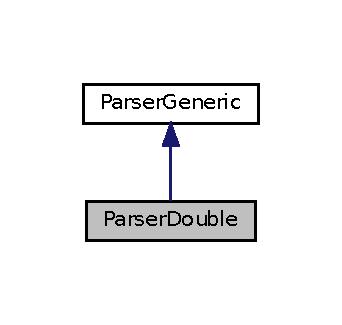
\includegraphics[width=164pt]{classParserDouble__inherit__graph}
\end{center}
\end{figure}


Collaboration diagram for Parser\+Double\+:
\nopagebreak
\begin{figure}[H]
\begin{center}
\leavevmode
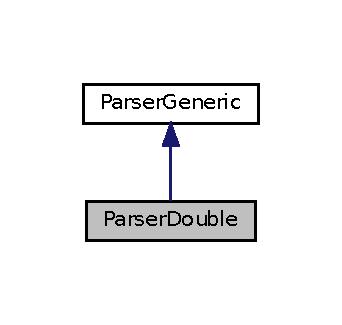
\includegraphics[width=164pt]{classParserDouble__coll__graph}
\end{center}
\end{figure}
\subsection*{Public Member Functions}
\begin{DoxyCompactItemize}
\item 
Object \hyperlink{classParserDouble_a45d2180f6c110f27347c95c2d207b462}{parse} (String s)
\end{DoxyCompactItemize}


\subsection{Detailed Description}
K\+Lasa tworząca parser konwertujący dane do typu Double implementująca interfejs \hyperlink{interfaceParserGeneric}{Parser\+Generic} \begin{DoxySeeAlso}{See also}
\hyperlink{interfaceParserGeneric}{Parser\+Generic} 

\hyperlink{classParser}{Parser} 
\end{DoxySeeAlso}


\subsection{Member Function Documentation}
\mbox{\Hypertarget{classParserDouble_a45d2180f6c110f27347c95c2d207b462}\label{classParserDouble_a45d2180f6c110f27347c95c2d207b462}} 
\index{Parser\+Double@{Parser\+Double}!parse@{parse}}
\index{parse@{parse}!Parser\+Double@{Parser\+Double}}
\subsubsection{\texorpdfstring{parse()}{parse()}}
{\footnotesize\ttfamily Object Parser\+Double.\+parse (\begin{DoxyParamCaption}\item[{String}]{s }\end{DoxyParamCaption})\hspace{0.3cm}{\ttfamily [inline]}}



Implements \hyperlink{interfaceParserGeneric_a42d671b89e41a5adb31a41c59db57503}{Parser\+Generic}.



The documentation for this class was generated from the following file\+:\begin{DoxyCompactItemize}
\item 
\hyperlink{ParserDouble_8java}{Parser\+Double.\+java}\end{DoxyCompactItemize}

\hypertarget{interfaceParserGeneric}{}\section{Parser\+Generic Interface Reference}
\label{interfaceParserGeneric}\index{Parser\+Generic@{Parser\+Generic}}


Inheritance diagram for Parser\+Generic\+:
\nopagebreak
\begin{figure}[H]
\begin{center}
\leavevmode
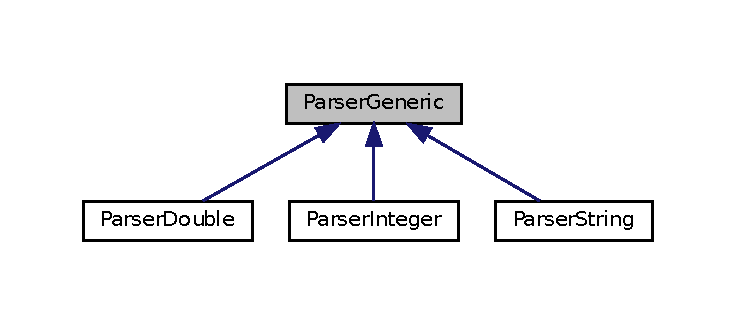
\includegraphics[width=350pt]{interfaceParserGeneric__inherit__graph}
\end{center}
\end{figure}
\subsection*{Public Member Functions}
\begin{DoxyCompactItemize}
\item 
Object \hyperlink{interfaceParserGeneric_a42d671b89e41a5adb31a41c59db57503}{parse} (String s)
\end{DoxyCompactItemize}


\subsection{Detailed Description}
Intefejs implementowany przez parsery odpowiednich typów 

\subsection{Member Function Documentation}
\mbox{\Hypertarget{interfaceParserGeneric_a42d671b89e41a5adb31a41c59db57503}\label{interfaceParserGeneric_a42d671b89e41a5adb31a41c59db57503}} 
\index{Parser\+Generic@{Parser\+Generic}!parse@{parse}}
\index{parse@{parse}!Parser\+Generic@{Parser\+Generic}}
\subsubsection{\texorpdfstring{parse()}{parse()}}
{\footnotesize\ttfamily Object Parser\+Generic.\+parse (\begin{DoxyParamCaption}\item[{String}]{s }\end{DoxyParamCaption})}



Implemented in \hyperlink{classParserDouble_a45d2180f6c110f27347c95c2d207b462}{Parser\+Double}, \hyperlink{classParserInteger_a56a141fdc62fbc8589b4259a0e65cbaa}{Parser\+Integer}, and \hyperlink{classParserString_a7054c77bf5579a99a7abf166aad1c640}{Parser\+String}.



The documentation for this interface was generated from the following file\+:\begin{DoxyCompactItemize}
\item 
\hyperlink{ParserGeneric_8java}{Parser\+Generic.\+java}\end{DoxyCompactItemize}

\hypertarget{classParserInteger}{}\section{Parser\+Integer Class Reference}
\label{classParserInteger}\index{Parser\+Integer@{Parser\+Integer}}


Inheritance diagram for Parser\+Integer\+:
\nopagebreak
\begin{figure}[H]
\begin{center}
\leavevmode
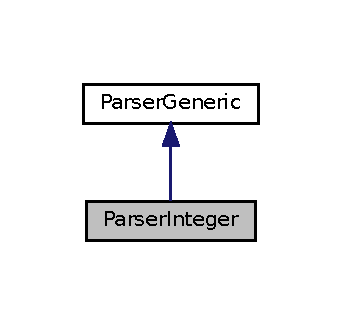
\includegraphics[width=164pt]{classParserInteger__inherit__graph}
\end{center}
\end{figure}


Collaboration diagram for Parser\+Integer\+:
\nopagebreak
\begin{figure}[H]
\begin{center}
\leavevmode
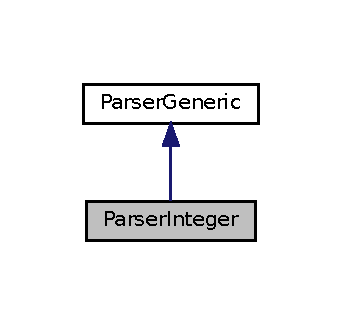
\includegraphics[width=164pt]{classParserInteger__coll__graph}
\end{center}
\end{figure}
\subsection*{Public Member Functions}
\begin{DoxyCompactItemize}
\item 
Object \hyperlink{classParserInteger_a56a141fdc62fbc8589b4259a0e65cbaa}{parse} (String s)
\end{DoxyCompactItemize}


\subsection{Detailed Description}
Klasa tworząca parser konwerujący string do typu Integer \begin{DoxySeeAlso}{See also}
\hyperlink{classParser}{Parser} 

\hyperlink{interfaceParserGeneric}{Parser\+Generic} 
\end{DoxySeeAlso}


\subsection{Member Function Documentation}
\mbox{\Hypertarget{classParserInteger_a56a141fdc62fbc8589b4259a0e65cbaa}\label{classParserInteger_a56a141fdc62fbc8589b4259a0e65cbaa}} 
\index{Parser\+Integer@{Parser\+Integer}!parse@{parse}}
\index{parse@{parse}!Parser\+Integer@{Parser\+Integer}}
\subsubsection{\texorpdfstring{parse()}{parse()}}
{\footnotesize\ttfamily Object Parser\+Integer.\+parse (\begin{DoxyParamCaption}\item[{String}]{s }\end{DoxyParamCaption})\hspace{0.3cm}{\ttfamily [inline]}}



Implements \hyperlink{interfaceParserGeneric_a42d671b89e41a5adb31a41c59db57503}{Parser\+Generic}.



The documentation for this class was generated from the following file\+:\begin{DoxyCompactItemize}
\item 
\hyperlink{ParserInteger_8java}{Parser\+Integer.\+java}\end{DoxyCompactItemize}

\hypertarget{classParserString}{}\section{Parser\+String Class Reference}
\label{classParserString}\index{Parser\+String@{Parser\+String}}


Inheritance diagram for Parser\+String\+:
\nopagebreak
\begin{figure}[H]
\begin{center}
\leavevmode
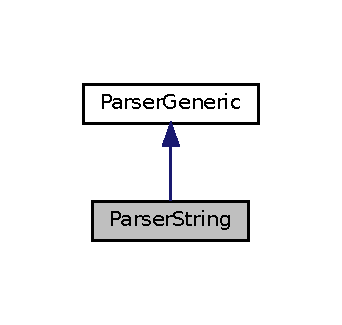
\includegraphics[width=164pt]{classParserString__inherit__graph}
\end{center}
\end{figure}


Collaboration diagram for Parser\+String\+:
\nopagebreak
\begin{figure}[H]
\begin{center}
\leavevmode
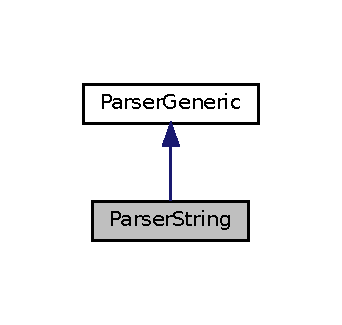
\includegraphics[width=164pt]{classParserString__coll__graph}
\end{center}
\end{figure}
\subsection*{Public Member Functions}
\begin{DoxyCompactItemize}
\item 
Object \hyperlink{classParserString_a7054c77bf5579a99a7abf166aad1c640}{parse} (String s)
\end{DoxyCompactItemize}


\subsection{Detailed Description}
Klasa tworząca parser konwerujący string do typu Double \begin{DoxySeeAlso}{See also}
\hyperlink{classParser}{Parser} 

\hyperlink{interfaceParserGeneric}{Parser\+Generic} 
\end{DoxySeeAlso}


\subsection{Member Function Documentation}
\mbox{\Hypertarget{classParserString_a7054c77bf5579a99a7abf166aad1c640}\label{classParserString_a7054c77bf5579a99a7abf166aad1c640}} 
\index{Parser\+String@{Parser\+String}!parse@{parse}}
\index{parse@{parse}!Parser\+String@{Parser\+String}}
\subsubsection{\texorpdfstring{parse()}{parse()}}
{\footnotesize\ttfamily Object Parser\+String.\+parse (\begin{DoxyParamCaption}\item[{String}]{s }\end{DoxyParamCaption})\hspace{0.3cm}{\ttfamily [inline]}}



Implements \hyperlink{interfaceParserGeneric_a42d671b89e41a5adb31a41c59db57503}{Parser\+Generic}.



The documentation for this class was generated from the following file\+:\begin{DoxyCompactItemize}
\item 
\hyperlink{ParserString_8java}{Parser\+String.\+java}\end{DoxyCompactItemize}

\hypertarget{classWindow}{}\section{Window$<$ T extends Comparable$<$ T $>$ Class Template Reference}
\label{classWindow}\index{Window$<$ T extends Comparable$<$ T $>$@{Window$<$ T extends Comparable$<$ T $>$}}


Inheritance diagram for Window$<$ T extends Comparable$<$ T $>$\+:
\nopagebreak
\begin{figure}[H]
\begin{center}
\leavevmode
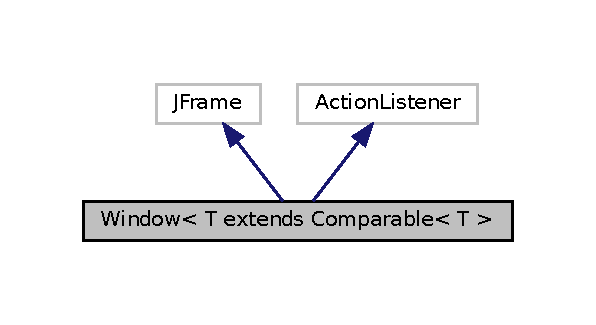
\includegraphics[width=286pt]{classWindow__inherit__graph}
\end{center}
\end{figure}


Collaboration diagram for Window$<$ T extends Comparable$<$ T $>$\+:
\nopagebreak
\begin{figure}[H]
\begin{center}
\leavevmode
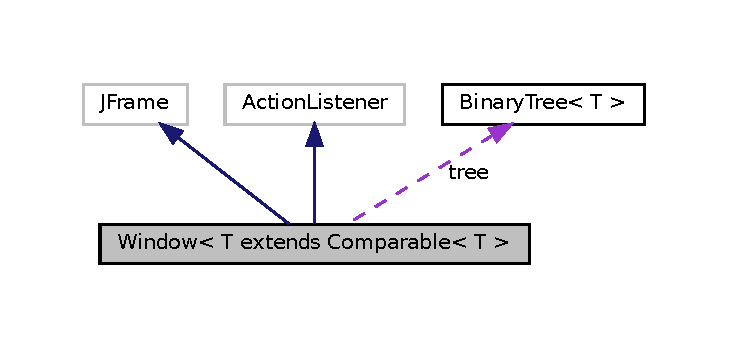
\includegraphics[width=350pt]{classWindow__coll__graph}
\end{center}
\end{figure}
\subsection*{Public Member Functions}
\begin{DoxyCompactItemize}
\item 
void \hyperlink{classWindow_aa0461cd99d9f9019c64d5e68dad1bead}{action\+Performed} (Action\+Event e)
\end{DoxyCompactItemize}


\subsection{Detailed Description}
Klasa okna służąca do wykonywania operacji na drzewie \begin{DoxySeeAlso}{See also}
\hyperlink{classBinaryTree}{Binary\+Tree} 

\hyperlink{classNode}{Node} 
\end{DoxySeeAlso}

\begin{DoxyParams}{Parameters}
{\em $<$\+T$>$} & typ naszego drzewa \\
\hline
\end{DoxyParams}


\subsection{Member Function Documentation}
\mbox{\Hypertarget{classWindow_aa0461cd99d9f9019c64d5e68dad1bead}\label{classWindow_aa0461cd99d9f9019c64d5e68dad1bead}} 
\index{Window@{Window}!action\+Performed@{action\+Performed}}
\index{action\+Performed@{action\+Performed}!Window@{Window}}
\subsubsection{\texorpdfstring{action\+Performed()}{actionPerformed()}}
{\footnotesize\ttfamily void \hyperlink{classWindow}{Window}$<$ T extends Comparable$<$ T $>$.action\+Performed (\begin{DoxyParamCaption}\item[{Action\+Event}]{e }\end{DoxyParamCaption})\hspace{0.3cm}{\ttfamily [inline]}}

Metoda służąca do nasłuuchiwania akcji Sprawdzamy który przycisk został wciśnięty i wykonujemy operacje W przypadku nieudanej operacji wyświetlamy okno dialogowe z błędem

Sprawdzamy, czy wierzchołek nie jest pusty 

The documentation for this class was generated from the following file\+:\begin{DoxyCompactItemize}
\item 
\hyperlink{Window_8java}{Window.\+java}\end{DoxyCompactItemize}

\chapter{File Documentation}
\hypertarget{BinaryTree_8java}{}\section{Binary\+Tree.\+java File Reference}
\label{BinaryTree_8java}\index{Binary\+Tree.\+java@{Binary\+Tree.\+java}}
\subsection*{Classes}
\begin{DoxyCompactItemize}
\item 
class \hyperlink{classBinaryTree}{Binary\+Tree$<$ T extends Comparable$<$ T $>$}
\end{DoxyCompactItemize}

\hypertarget{Main_8java}{}\section{Main.\+java File Reference}
\label{Main_8java}\index{Main.\+java@{Main.\+java}}
\subsection*{Classes}
\begin{DoxyCompactItemize}
\item 
class \hyperlink{classMain}{Main}
\end{DoxyCompactItemize}

\hypertarget{Node_8java}{}\section{Node.\+java File Reference}
\label{Node_8java}\index{Node.\+java@{Node.\+java}}
\subsection*{Classes}
\begin{DoxyCompactItemize}
\item 
class \hyperlink{classNode}{Node$<$ T $>$}
\end{DoxyCompactItemize}

\hypertarget{Parser_8java}{}\section{Parser.\+java File Reference}
\label{Parser_8java}\index{Parser.\+java@{Parser.\+java}}
\subsection*{Classes}
\begin{DoxyCompactItemize}
\item 
class \hyperlink{classParser}{Parser$<$ T $>$}
\end{DoxyCompactItemize}

\hypertarget{ParserDouble_8java}{}\section{Parser\+Double.\+java File Reference}
\label{ParserDouble_8java}\index{Parser\+Double.\+java@{Parser\+Double.\+java}}
\subsection*{Classes}
\begin{DoxyCompactItemize}
\item 
class \hyperlink{classParserDouble}{Parser\+Double}
\end{DoxyCompactItemize}

\hypertarget{ParserGeneric_8java}{}\section{Parser\+Generic.\+java File Reference}
\label{ParserGeneric_8java}\index{Parser\+Generic.\+java@{Parser\+Generic.\+java}}
\subsection*{Classes}
\begin{DoxyCompactItemize}
\item 
interface \hyperlink{interfaceParserGeneric}{Parser\+Generic}
\end{DoxyCompactItemize}

\hypertarget{ParserInteger_8java}{}\section{Parser\+Integer.\+java File Reference}
\label{ParserInteger_8java}\index{Parser\+Integer.\+java@{Parser\+Integer.\+java}}
\subsection*{Classes}
\begin{DoxyCompactItemize}
\item 
class \hyperlink{classParserInteger}{Parser\+Integer}
\end{DoxyCompactItemize}

\hypertarget{ParserString_8java}{}\section{Parser\+String.\+java File Reference}
\label{ParserString_8java}\index{Parser\+String.\+java@{Parser\+String.\+java}}
\subsection*{Classes}
\begin{DoxyCompactItemize}
\item 
class \hyperlink{classParserString}{Parser\+String}
\end{DoxyCompactItemize}

\hypertarget{Window_8java}{}\section{Window.\+java File Reference}
\label{Window_8java}\index{Window.\+java@{Window.\+java}}
\subsection*{Classes}
\begin{DoxyCompactItemize}
\item 
class \hyperlink{classWindow}{Window$<$ T extends Comparable$<$ T $>$}
\end{DoxyCompactItemize}

%--- End generated contents ---

% Index
\backmatter
\newpage
\phantomsection
\clearemptydoublepage
\addcontentsline{toc}{chapter}{Index}
\printindex

\end{document}
